\RequirePackage[l2tabu, orthodox]{nag}
\documentclass[a4paper]{article}
\usepackage[utf8]{inputenc}
\usepackage[T1]{fontenc}
\usepackage{lmodern}
\usepackage[pdftex, hidelinks,
            pdftitle={Flödesanimering i Realtid med 3-D Curlbrus},
            pdfauthor={Martin Estgren and and Rasmus Hedin and Alfred Rundquist and Erik S. V. Jansson},
            pdfsubject={Computer Graphics -- Animation -- Physical Simulation / Procedural Animation},
            pdfkeywords={curl-noise,animation,fluid simulation,navier-stokes,gpu,real-time}]{hyperref}

\usepackage{bm}
\usepackage{caption}
\usepackage{listings}
\usepackage{mathtools}
\usepackage[margin=0.8in]{geometry}
\usepackage[parfill]{parskip}
\usepackage[swedish]{babel}
\usepackage{algorithmic}
\usepackage{graphicx}
\usepackage{courier}
\usepackage{hyperref}
\usepackage{amsmath}
\usepackage{amssymb}
\usepackage{algorithm}
\usepackage{multicol}
\setlength{\columnsep}{0.5cm}
\usepackage[capitalize, noabbrev]{cleveref}
\usepackage[activate={true, nocompatibility}, final,
            tracking=true, kerning=true, spacing=true,
            factor=1100, stretch=10, shrink=10]{microtype}

\DeclareCaptionFormat{modifiedlst}{\rule{\textwidth}{0.85pt}\\[-2.9pt]#1#2#3}
\captionsetup[lstlisting]{format =  modifiedlst,
labelfont=bf,singlelinecheck=off,labelsep=space}
\lstset{basicstyle=\footnotesize\ttfamily,
        breakatwhitespace = false,
        breaklines = true,
        keepspaces = true,
        language = C++,
        showspaces = false,
        showstringspaces = false,
        frame = tb,
        numbers = left,
        numbersep = 5pt,
        xleftmargin = 16pt,
        framexleftmargin = 16pt,
        belowskip = \bigskipamount,
        aboveskip = \bigskipamount,
        escapeinside={<@}{@>}}

\date{\vspace{-0.5ex}} % Buys us some space.
\title{\vspace{-2.2cm}\textbf{Flödesanimering i Realtid med 3-D Curlbrus}\\
       \Large{\textit{--- en kort teknisk saga angående dess fasor och dess under ---}}\vspace{-0.25cm}}
\author{{\textbf{Martin Estgren}}\;\;\;\;\;\; {\href{mailto:mares480@student.liu.se}{\texttt{<mares480@student.liu.se>}}}\\
        {\textbf{Rasmus Hedin}}\;\;\;\;\;\;\;\; {\href{mailto:rashe877@student.liu.se}{\texttt{<rashe877@student.liu.se>}}}\\
        {\textbf{Alfred Rundquist}}\;\;\; {\href{mailto:alfru536@student.liu.se}{\texttt{<alfru536@student.liu.se>}}}\\
        {\textbf{Erik S. V. Jansson}}\; {\href{mailto:erija578@student.liu.se}{\texttt{<erija578@student.liu.se>}}}}

\begin{document}
    \maketitle
\begin{multicols}{2}

    \section{Introduktion}

    Ett viktigt område inom \emph{datorgrafik och visualisering} är förmågan att \emph{simulera}/\emph{animera} verklighetstrogna \emph{flödessystem} i \emph{realtid}. Dessa används i bl.a. spel och filmer för att enkelt skapa \emph{visuella effekter} som t.ex. \emph{rök- och vattenrörelser}; effekter som vanligtvis inte görs ``för hand'', och är mer lämpliga att genereras av en dator. I detta projekt har vi implementerat ett \emph{grundläggande flödessystem} för att \emph{animera ett partikelsystem} i 3-D med hjälp av den så kallade \emph{Curl-Noise} (``curlbrus''), först presenterad av \emph{Bridson et al.}~\cite{bridson2007curl} i 2007.

    \textit{Curlbrus} används för att framställa verklighetstrogna \emph{partikelflöden} genom att procedurellt animera \emph{turbulenta flöden}. Detta görs genom att använda ett \emph{procedurellt brus} för att skapa ett \emph{divergens-fritt vektorfält}. Detta är ett billigare alternativ till \emph{Navier-Stokes}, som är fysiskt korrekt; men eftersom vi endast är efter dess visuella egenskaper, är Curlbrus tillräckligt bra. Dessutom kan Curlbrus beräknas i realtid, vilket gör den lämplig för integrering i t.ex. spel och infovis.

    Målet med detta projekt var att skapa ett enkelt \emph{3-D partikelsystem} där partiklarnas rörelse bestäms av ett vektorfällt genererat genom \emph{Curlbrus metoden} tillsammans med några enkla visuella effekter.

    Den preliminära arbetsprocessen gick ut på att vi parprogrammera med versionshantering via \textit{Git}. För att realisera partikelsystemet valde vi att använda \textit{OpenCL} för partikelberäkningar, \textit{OpenGL} för rendering, \textit{GLFW} för fönsterhantering, \textit{AntTweakbar} för ``run-time'' konfigurering, och \textit{GLEW} för att hantera \textit{OpenGL}-tillägg. Själva koden skrevs i C++, där våra kernels skrevs i \textit{OpenCLs} variant av C, samt shaders i \textit{GLSL}.

    \vspace{-0.5cm}
    \section{Teori och metodik}
    \vspace{-0.3cm}
    \subsection{Systemöversikt} \label{sec:system}

    Vid tidpunkten \(t_n\) befinner sig varje partikel vid sin egen position \(\vec{x}\), lagrade i en \emph{buffer}. Målet är att räkna ut partikelns nästa position \(\vec{x}'\) vid tidpunkten \(t_{n+1}\) (d.v.s. vi stegar fram simuleringen). Detta görs genom \(\vec{x}' = \vec{x} + \mathbf{\hat{V}}(\vec{x})\), där \(\mathbf{\hat{V}}(\vec{x})\) är \emph{fältriktningen}. Allt detta hanteras av \emph{partikelsystemet}, där dessutom \(\mathbf{\hat{V}}(\vec{x})\) skapas, och beskrivs under Rubrik~\ref{sec:partikelsystemet}. Detta görs parallellt på GPU:n för varje partikel under samma \(t_n\). Vilket gör att positionerna \(\vec{x}'\) kan återanvändas när vi ska \emph{visualisera} dem med \emph{partikelrenderaren}, då båda systemen ej behöver lämna grafikprocessorns minnesrymd. Detta leder till god prestanda, och arbetstypen passar dessutom bra till sådana typer av processorer då synkroniseringen är minimal. Se Figur~\ref{fig:system}.

    \begin{figure}[H]
    \center
    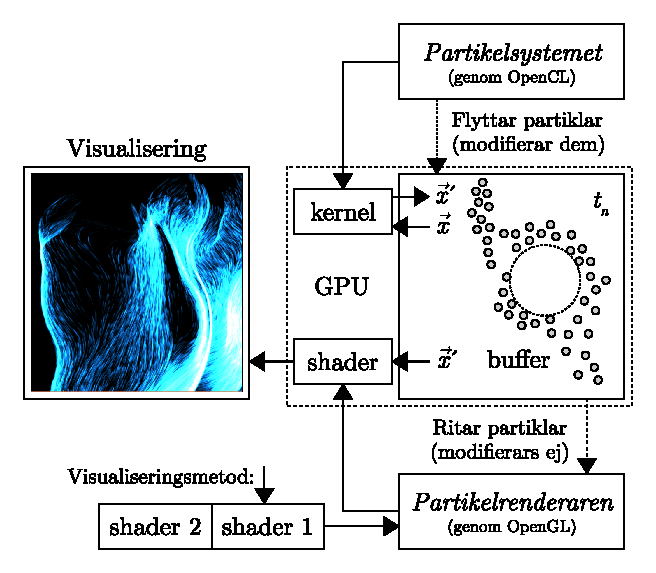
\includegraphics[width=0.5\textwidth]{share/System.eps}
    \caption{konceptuell översikt över våra två subsystem.}
    \label{fig:system}
    \end{figure}

    Detta görs genom att ladda upp en \emph{kernel} (beräkningskärna) som läser in \(\vec{x}\) och därefter skriver över denna med \(\vec{x}'\). Genom att läsa \(\vec{x}'\) från den delade buffern så kan en \emph{shader} användas för att rita partiklarna, genom att tolka hela \(\vec{x}'\) som en \emph{vertex buffer}. Man kan enkelt ändra \emph{visualiseringsmetod} (hur man ritar \(\vec{x}'\)) genom att byta shader, vilket beskrivs under Rubrik~\ref{sec:partikelrenderaren}.

    \vspace{-0.35cm}
    \subsection{Partikelsystemet} \label{sec:partikelsystemet}

    Partikelsystemet bygger på att varje partikels nästkommande position beräknas parallellt genom en \textit{OpenCL} kernel för varje frame. 

    Originalpapperet presenterar både riktningsberäkningarna för två och tre dimensioner men eftersom vi valt att enbart implementera den sistnämnda fokuserar vi på den. Vi kommer ej heller följa originalpapperets beräkningar exakt utan justerar beroende på vad som passar vårat system bättre.

    I korthet kan man säga att vi producerar tre olika vektorfält som vi kombinerar. De första två fälten representerar turbulensen och den allmänna riktningen som partiklarna ska följa. Dessa kombineras genom att adderas. Efter detta modifieras resultatfältet så att partiklarna åker runt solida kroppar och slutligen applicerar vi en rotationsoperation (curl) vilket resulterar i ett divergensfritt vektorfält.

\begin{figure}[H]
\begin{minipage}[]{0.5\textwidth}
\center

\includegraphics[width=0.48\textwidth]{share/Noise_downscale.png}

\includegraphics[width=0.48\textwidth]{share/Background_downscale.png}

\vspace{0.1cm}


\includegraphics[width=0.48\textwidth]{share/Alpha_downscale.png}
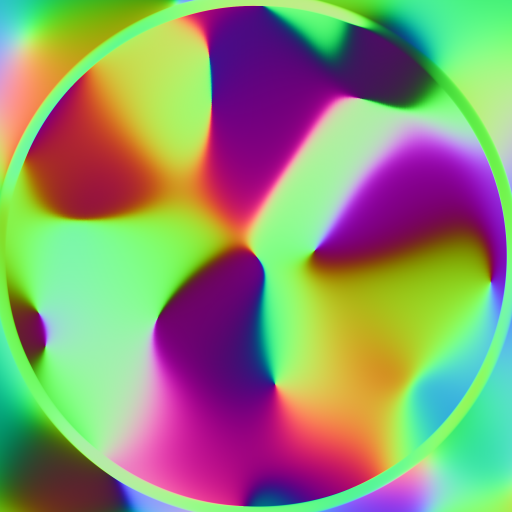
\includegraphics[width=0.48\textwidth]{share/Curl_downscale.png}
\end{minipage}
    \caption{$xy$-plan genomskärningar av  a) \emph{turbulensfältet} b) \emph{bakgrundsfältet} c) \emph{rampfunktionen} d) \emph{riktningsfältet}. (i den ordningen som visas: vänster$\rightarrow$höger, upp$\rightarrow$ner)}
\label{fig:curlnoise}
\end{figure}

\vspace{-0.3cm}
    \textbf{Turbulensfältet}

    Turbulensfältet beräknas genom att sampla en procedurell brusfunktion. Vi valde att använda \textit{Simplex noise}\footnote{\url{https://github.com/stegu/perlin-noise/blob/master/src/simplexnoise1234.c}} vilket förklaras i detalj av \emph{Stefan Gustavsson}~\cite{gustavson2005simplex}. Brusfunktionen samplas runt varje partikels position enligt följande funktion.
    \begin{equation}
   \vec{N}(\vec{x}) =
        \begin{pmatrix}
        n((\vec{x} + \vec{\epsilon}_x)/L)
        \\
        n((\vec{x} + \vec{\epsilon}_y)/L)
        \\ 
        n((\vec{x} + \vec{\epsilon}_z)/L)
        \end{pmatrix} * \gamma M_nL
    \end{equation}
    Där $\vec{\epsilon}$ representerar en förskjutning så att alla vektorkomponenter inte blir korrelerade, i detta fall $\vec{\epsilon} = \begin{pmatrix}
8 & 0 & 0\\ 
0 & 8 & 0\\ 
0 & 0 & 8
\end{pmatrix}$. $n(\vec{x})$ är brusfunktionen som samplas för att producera turbulens i fältet. $\gamma$ representerar förhållande mellan brus och bakgrundsfält där $0$ är inget brus och därmed ingen turbulens medan $1$ är fullt brus utan något bakgrundsfält. $M_n$ är styrkan på bruset (fältriktningen är normerad så vi skalar upp det till vad vi vill ha). $L$ är längdskalan på bruset vilket i vårat fall är relativt stor (20-100) då vi vill ha långa övergångar i bruset.

\textbf{Bakgrundsriktningen}

Bakgrundsriktningen representerar den generella riktningen vi vill att partiklarna ska följa. Detta beskrivs inte något vidare i referensartikeln. Vi valde istället att anpassa en redan existerande implementation\footnote{\url{https://github.com/kbladin/Curl_Noise/blob/master/shaders/point_cloud_programs/update_velocities_curl_noise.frag}} av K. Bladin, vilket resulterar i ett bakgrundsfält som går i en uniform riktning efter att $\nabla \times$ operatorn har applicerats.
\begin{equation}
     \vec{F}(\vec{x}) = (1.0-\gamma) *  \vec{D}(\vec{x}) * M_f
\end{equation}
$ \vec{D}(\vec{x})$ representerar fältriktningen i den angivna punkten och $M_f$ är magnituden vi vill ha. Fältriktningen är beräknad enligt följande formel
\begin{equation}
    \vec{D}(\vec{x}) = \vec{x} \times \vec{p}
\end{equation}
Där $\vec{p}$ är fältriktningen vi vill att partiklarna ska följa.


Turbulensfältet adderas med bakgrundsriktningen ($\vec{\psi} = \vec{N}(\vec{x}) + \vec{F}(\vec{x})$) för att sedan justeras så att partiklarna beaktar solida sfärer utplacerade i vektorfältet. 

\textbf{Solida kroppar i fältet}

För att få alla partiklar att respektera de sfärer vi placerat i fältet använder vi rampfunktionen
\begin{equation}
ramp(r) = \left\{\begin{matrix}
1  && r > 1
\\
6r^4 - 15r^4 + 10r^3 && 0 \le r \le 1
\\ 
0  && r < 0
\end{matrix}\right.
\end{equation}
där $r$ är distansen $\vec{x}$ till närmaste sfär delat på distansen av sfären inflytande. 

Resultatet från rampfunktionen som $\alpha = | ramp(d(\vec{x})/d_0) |$ där $d_0$  är en arbiträr skalfaktor. Slutligen beräknar vi hur fältet runt sfärer se ut genom 
\begin{equation}
\vec{\psi}_c(\vec{x}) = \alpha * \vec{\psi}(\vec{x}) + (1.0 - \alpha) * \hat{n} * \vec{\psi}(\vec{x}) \cdot \hat{n}
\end{equation}
där $\hat{n}$ är normalen från $\vec{x}$ till den närmsta sfären. Detta producerar en övergång från fältriktningen till en riktning tangentiell mot sfären.

\textbf{Curl}

Vi får fram $ \nabla \vec{\psi}$ genom en \textit{finit differensmetod}
\begin{equation}
\vec{vx} = \vec{\psi}_c(\vec{x} + \vec{\epsilon}_x  ) - \vec{\psi}_c(\vec{x} - \vec{\epsilon}_x  )
\end{equation}
\begin{equation}
\vec{vy} = \vec{\psi}_c(\vec{x} + \vec{\epsilon}_y  ) - \vec{\psi}_c(\vec{x} - \vec{\epsilon}_y  )
\end{equation}
\begin{equation}
\vec{vz} = \vec{\psi}_c(\vec{x} + \vec{\epsilon}_z  ) - \vec{\psi}_c(\vec{x} - \vec{\epsilon}_z  )
\end{equation}
där $\vec{\epsilon} = \begin{pmatrix}
0.0001 & 0 & 0\\ 
0 & 0.0001 & 0\\ 
0 & 0 & 0.0001
\end{pmatrix}$ och varje resultatvektor $\vec{vx},\vec{vy},\vec{vz}$ är de partiella derivatorna i punkten $\vec{x}$.

Slutligen beräknas den slutgiltiga fältriktningen genom att applicera curl operatorn på vår framtagna gradient genom
\begin{equation}
\mathbf{\hat{V}}(\vec{x}) =
\nabla \times \begin{pmatrix}
\vec{vy}_z - \vec{vz}_y
\\ 
\vec{vz}_z - \vec{vx}_y
\\ 
\vec{vx}_z - \vec{vy}_y
\end{pmatrix} / 0.0002
\end{equation}
och normeras så att vi själva kan bestämma vad hastigheten för partiklarna ska vara. En genomskärning i $xy$-planet av dessa fält kan ses i Figur~\ref{fig:curlnoise}.

\subsection{Partikelrenderaren} \label{sec:partikelrenderaren}

Då varje position \(\vec{x}\) finns tillgänglig i \emph{vertex shadern} (enligt Rubrik~\ref{sec:system}) kan vi ändra hur de ritas ut genom att modifiera senare \emph{shader ``pipeline'' steg}. Tre styckna olika visualiseringsmetoder har implementerats, som beskrivs individuellt i kommande delar. Dessutom har vi valt att använda \emph{additiv färgblandning} när vi skriver till skärmbufferten, främst av estetiska skäl (områden med fler partiklar ger ett intryck att det är ``ljusare''), men dessutom av rent praktiska skäl (som kommer förklaras i kommande delar). Bilder över dessa visualiseringsmetoder finns i Rubrik~\ref{sec:results}.

\textbf{Punktvisualiseringen}

Den enklaste typen av visualisering är att bara skapa en ``punkt'' där partikeln bör ligga. Här behöver vi endast en \emph{vertex shader} och en \emph{fragment shader}. Då användaren ska kunna observera scenen från flera håll, måste positionerna \(\vec{x}\) omvandlas till det korrekta koordinatsystemet, \(\mathbf{MVP}\vec{x}\) i \emph{vertex shadern}. Därefter ger vi punkten en enkel färg genom att sätta resultatet från \emph{fragment shadern} till \(\begin{bmatrix}|x| & |y| & |z| & 1.0\end{bmatrix}\). Det vill säga, färgen av partikeln ges av dess position \(\vec{x}\).

\textbf{Billboardsvisualiseringen}

Visuella effekter så som eld och rök kan enkelt representeras med hjälp av s.k. \emph{``billboards''} (alt. \emph{``impostors''}), som är ett texturerat plan som alltid är riktad mot åskådaren (vilket ger intrycket att den är 2-D). Detta görs enligt \emph{Ingemar Ragnemalm}~\cite{ragnemalm2008polygons} genom att: \[\mathbf{M} = \begin{bmatrix} 1 & 0 & 0 & x \\
                                    0 & 1 & 0 & y \\
                                    0 & 0 & 1 & z \\
                                    0 & 0 & 0 & 1 \end{bmatrix}, \;
          \vec{x} = \begin{bmatrix}x & y & z\end{bmatrix}.\]

Hur skapas detta plan dock, given en punkt \(\vec{x}\)? Då vi har valt att göra allt detta i våra shaders, måste vi \emph{skapa ny geometri} under körtid. Man gör detta med hjälp av en s.k. \emph{geometry shader}, ett steg som ligger mellan en \emph{vertex shader} och en \emph{fragment shader}.

\vspace{-0.3cm}
\begin{figure}[H]
\center
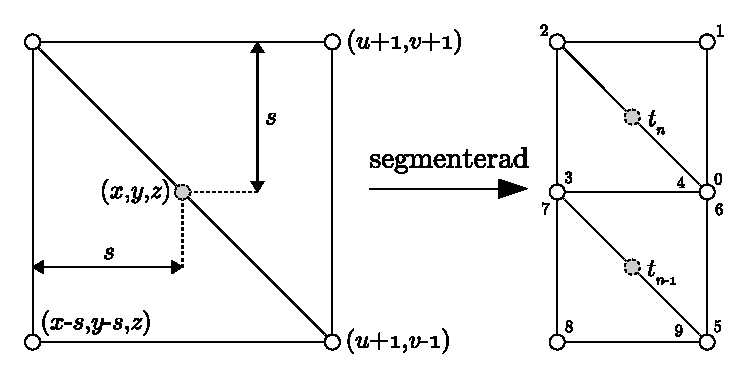
\includegraphics[width=0.5\textwidth]{share/Billboards.eps}
\caption{(a) en billboard (b) segmenterade billboards.}
\label{fig:bill}
\end{figure}
\vspace{-0.3cm}

Som figur~\ref{fig:bill}~(a) visar, skapar våran geometry shader för varje punkt \(\vec{x}\) (representerad som en grå cirkel i figuren), 4st nya hörn centrerade runt \(\vec{x}\) (de vita cirklarna) genom \texttt{EmitVertex}. Dessa flyttats med \(s\) enheter åt respektive håll; en parameter som bestämmer hur stor planet ska vara. Man genererar primitiver (trianglar i detta fall) genom att anropa \texttt{EndPrimitive}. Sist sätter vi \((u, v)\)-koordinaterna för de hörn vi skapat, och använder dessa i \emph{fragment shadern} för att rita ut en 2-D textur som har ``häftats'' till/på vårat plan.

\textbf{Vektorfältvisualiseringen}

För att enklare kunna visualisera riktningsfältet har vi implementerat \emph{``glyphs''}, som bl.a. beskrivs i \emph{McQuinn et al.}~\cite{mcquinn2013glyphsea}. Tekniken går ut på att ``dra ut'' en billboard så att den följer fältets riktning. Vi har gjort en förenklad variant, där de \(k\):st senaste \(\vec{x}\)-värden (vid tidsteg \(t_{n-1}, ..., t_{n-k}\)) lagras i en \emph{cirkulär buffer} \(\mathcal{C}\). Dessa används för att skapa en \emph{segmenterad billboard}, där de olika segmenten skapas mellan två punkter \(\vec{x}_{i-1}\),~\(\vec{x}_i\), där \(\vec{x}_{i-1}\),~\(\vec{x}_i\)~\(\in \mathcal{C}\). För varje segment skapas två hörn vid sidan av \(\vec{x}_i\) och två hörn vid sidan av \(\vec{x}_{i-1}\) enligt figur~\ref{fig:bill}~(b), som sedan används för att generera primitiver för varje segment (som kopplas samman).

\subsection{De övriga teknikaliteterna}

\clearpage

\section{Resultat \& diskussion} \label{sec:results}

\begin{figure}[H]
\center
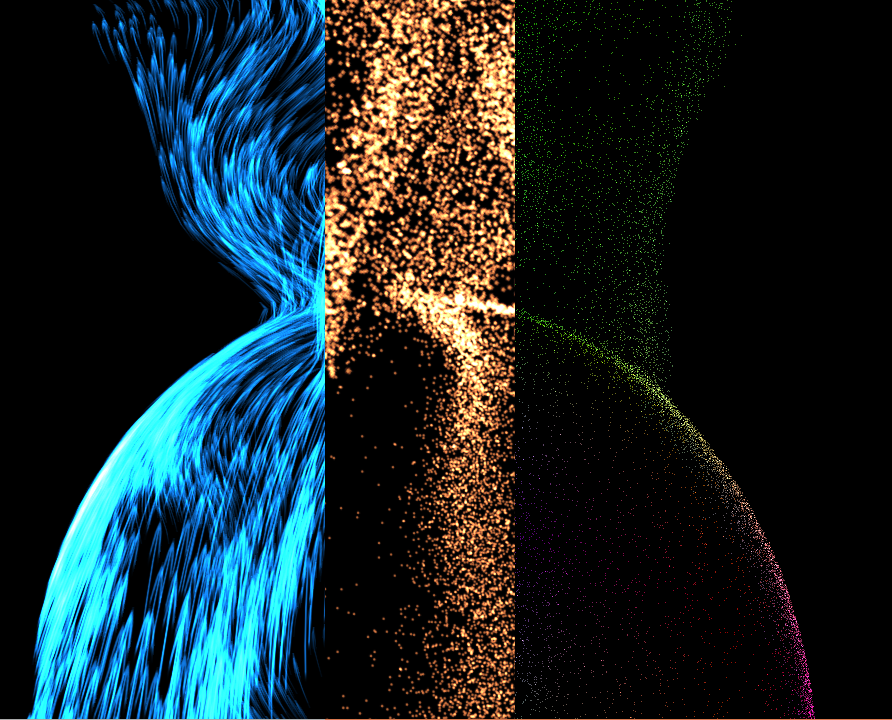
\includegraphics[width=0.48\textwidth]{share/merged_shaders.png}
    \caption{visualisering av \emph{partikelsystemet} med tre olika metoder: \emph{vektorfält-}, \emph{billboard-}, och \emph{punktvisualisering} som drivs av \emph{partikelrenderaren}. Scenariot innehåller en solid sfärisk kropp och med en längdskala på \(L\approx20\).}
\label{fig:verysexy}
\end{figure}

        \subsection{Problem samt lösningar}

            \textbf{``Svarta hål'' av ej divergens-frihet}

            % ...

            \textbf{Interpoleringsfel av CPU Simplex}

            % ...

            \textbf{Konstigheter i ``geometry shader''}

            % ...

            \textbf{Utföra mjuka kamera övergångar}

            % ...

            \textbf{Hämska fulhack för ``callbacks'' }

            % ...

        \subsection{Framtida förbättringar}

            \textbf{Segmentering med ``B-splines''}

            % ...

            \textbf{Filformat för ``egna'' scenarion}

            % ...

            \textbf{Konkreta scenarion av shaders}

            % ...

        \subsection{Projektreflektioner}

    \nocite{*} % Include all.
    \bibliographystyle{abbrv}
    \bibliography{cnpf}
\end{multicols}
\end{document}
